\documentclass[conference]{IEEEtran}

\usepackage{cite}
\usepackage{amsmath,amssymb}
\usepackage{graphicx}
\usepackage{booktabs}
\usepackage{array}
\usepackage{url}
\usepackage{tikz}
\usetikzlibrary{arrows.meta,positioning,fit,backgrounds,shapes.geometric}

\begin{document}

\title{PulseCI: Design and Implementation of an Automated Continuous Integration Pipeline for Python Applications}

\author{
\IEEEauthorblockN{Chethana Sri}
\IEEEauthorblockA{
Department of Computer Technology\\
Madras Institute of Technology\\
Anna University, Chennai, India\\
chethanasriadusumalli@gmail.com
}
}
\maketitle

\begin{abstract}
Continuous Integration (CI) is a software engineering practice in which code changes are integrated frequently and validated through automated processes. Without repeatable validation, defects may remain undetected until later development stages, while manual testing can make feedback inconsistent. This paper presents PulseCI, a Python-oriented automated Continuous Integration pipeline. The paper describes a staged workflow for receiving source changes, preparing the execution environment, validating project inputs, running configured checks and tests, and reporting execution outcomes. A layered architecture is presented to distinguish the source-control trigger, pipeline orchestration, execution stages, and feedback path. The system is evaluated through functional scenarios covering pipeline initialization, validation, dependency handling, test execution, and failure reporting. The paper deliberately distinguishes implemented functionality from proposed extensions; quantitative claims are not made without measured experimental data.
\end{abstract}

\begin{IEEEkeywords}
Continuous Integration, DevOps, Python, Automation, Software Testing, Pipeline Orchestration, Git
\end{IEEEkeywords}

\section{Introduction}
Modern software projects evolve through frequent source-code changes. Each change can introduce syntax errors, dependency conflicts, regressions, or integration defects. If validation is postponed until a later development phase, diagnosing the cause of a failure can become more difficult.

Continuous Integration (CI) addresses this problem by integrating changes frequently and executing automated validation as part of the development workflow. Fowler describes CI as a practice centered on frequent integration and automated build verification \cite{fowler}. Empirical research has examined both the benefits and the implementation challenges of CI, including its effects on development activities and quality assurance \cite{soares, hilton}.

This paper presents PulseCI, a Python-focused CI project intended to organize software validation into a repeatable pipeline. The paper's contributions are:
\begin{itemize}
    \item a layered architecture separating source changes, pipeline coordination, execution stages, and feedback;
    \item a staged workflow for project validation, dependency preparation, and automated testing, subject to the actual project configuration;
    \item a functional evaluation structure for recording successful and unsuccessful pipeline scenarios.
\end{itemize}

\section{Related Work}
Fowler's discussion of Continuous Integration emphasizes frequent integration and rapid feedback from automated verification \cite{fowler}. Humble and Farley describe continuous delivery practices that extend automated build and test processes toward reliable release workflows \cite{humble}. Kim \textit{et al.} discuss the organizational and technical practices associated with DevOps, including automation and collaboration across development and operations \cite{kim}.

Soares \textit{et al.} conducted a systematic literature review of empirical studies on CI. Their review identifies effects across development activities, software processes, quality assurance, integration patterns, defects, and build practices \cite{soares}. Hilton \textit{et al.} studied the adoption of CI in open-source projects and reported that CI services can help developers detect problems during development \cite{hilton}. Research on continuous integration, delivery, and deployment has also examined the approaches, tools, challenges, and practices involved in adopting these workflows \cite{shahin}.

In the implementation ecosystem, Git provides distributed version control \cite{git}. pytest provides a Python testing framework for writing and executing automated tests \cite{pytest}. GitHub Actions documents event-triggered workflows composed of jobs and steps, illustrating a widely used model for repository-based automation \cite{actions}. These tools and practices provide context for the design of PulseCI; they are not all claimed as internal components unless they are present in the actual implementation.

\section{Problem Statement and Objectives}
\subsection{Problem Statement}
Manual validation of code changes can be repetitive and inconsistent. A developer may forget to run a particular check, use a different environment, or overlook a failing test. A repeatable pipeline can centralize configured validation tasks and provide a consistent execution result.

\subsection{Objectives}
The objectives of PulseCI are to:
\begin{itemize}
    \item organize software validation into clearly defined pipeline stages;
    \item automate the checks and tests configured by the project;
    \item provide execution feedback that helps identify failed stages;
    \item support repeatable validation of Python application changes.
\end{itemize}

\section{Proposed System}
PulseCI is presented as a pipeline that coordinates a sequence of validation activities. At a conceptual level, a source-code change initiates a pipeline run. The pipeline prepares the project environment, performs configured validation, invokes automated tests, collects process outcomes, and reports a final status.

The exact trigger mechanism, commands, dependency manager, and reporting interface must match the implementation. The architecture in Fig.~\ref{fig:architecture} therefore shows functional roles rather than assuming a particular hosting service or deployment platform.

\subsection{System Architecture}
The architecture is divided into four logical layers:
\begin{enumerate}
    \item \textbf{Source layer:} the developer modifies code and records changes in a Git repository.
    \item \textbf{Trigger and orchestration layer:} a configured trigger starts PulseCI, which coordinates the pipeline stages.
    \item \textbf{Execution layer:} project validation, environment/dependency preparation, and automated tests are executed in sequence or as configured.
    \item \textbf{Feedback layer:} stage outputs and exit statuses are collected and presented as a pipeline result.
\end{enumerate}

\begin{figure*}[!t]
\centering
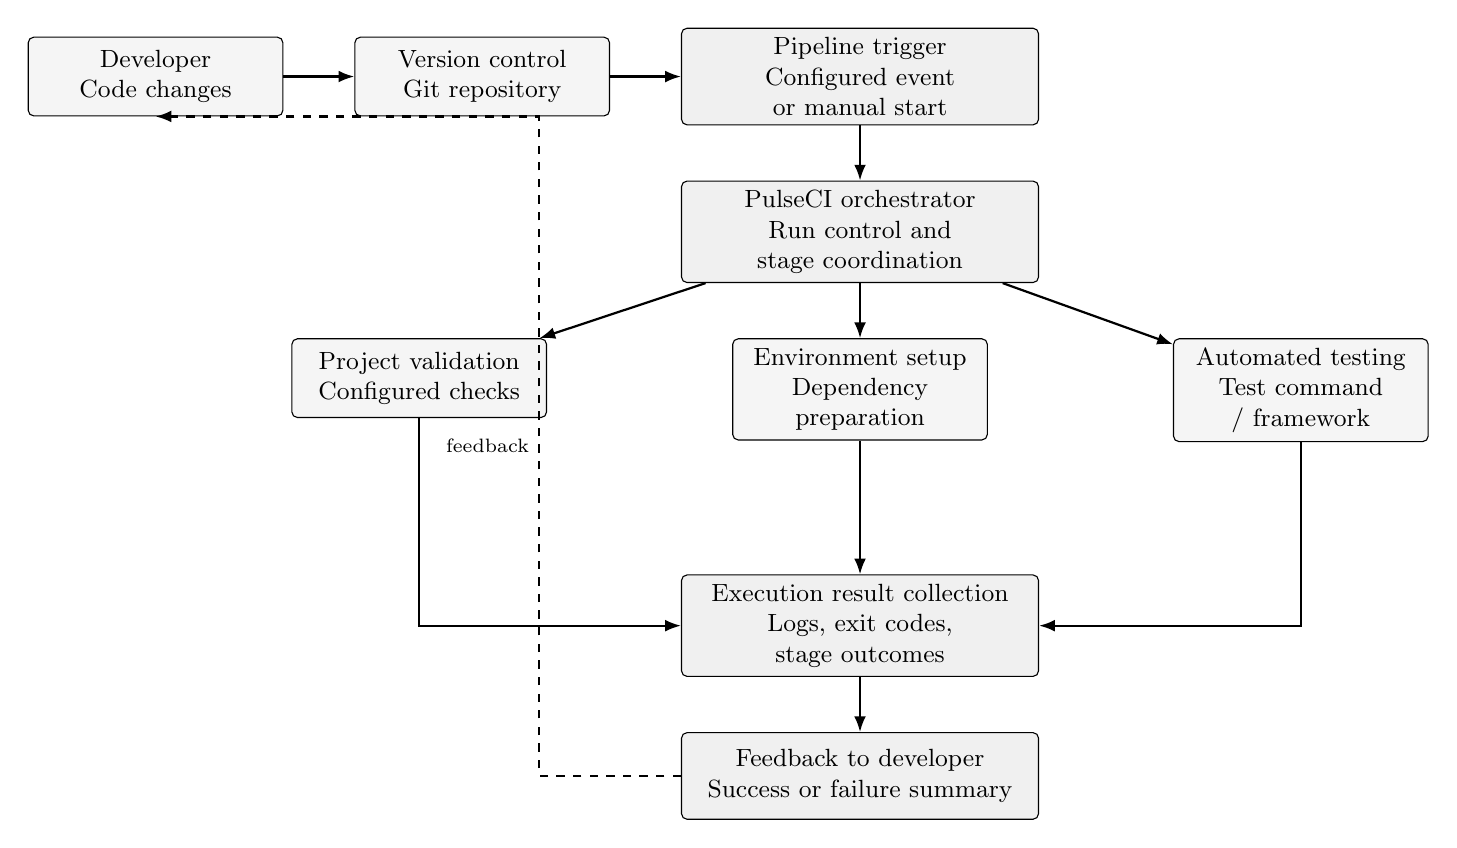
\begin{tikzpicture}[
  font=\small,
  node distance=7mm and 9mm,
  block/.style={draw, rounded corners=2pt, align=center, minimum height=10mm, text width=30mm, fill=gray!8},
  wide/.style={draw, rounded corners=2pt, align=center, minimum height=11mm, text width=43mm, fill=gray!12},
  arrow/.style={-{Latex[length=2mm]}, thick},
  dashedarrow/.style={-{Latex[length=2mm]}, thick, dashed}
]
\node[block] (dev) {Developer\\Code changes};
\node[block, right=of dev] (git) {Version control\\Git repository};
\node[wide, right=of git] (trigger) {Pipeline trigger\\Configured event or manual start};
\node[wide, below=of trigger] (engine) {PulseCI orchestrator\\Run control and stage coordination};

\node[block, below left=of engine, xshift=-8mm] (validate) {Project validation\\Configured checks};
\node[block, below=of engine] (deps) {Environment setup\\Dependency preparation};
\node[block, below right=of engine, xshift=8mm] (tests) {Automated testing\\Test command / framework};

\node[wide, below=17mm of deps] (collector) {Execution result collection\\Logs, exit codes, stage outcomes};
\node[wide, below=of collector] (report) {Feedback to developer\\Success or failure summary};

\draw[arrow] (dev) -- (git);
\draw[arrow] (git) -- (trigger);
\draw[arrow] (trigger) -- (engine);
\draw[arrow] (engine) -- (validate);
\draw[arrow] (engine) -- (deps);
\draw[arrow] (engine) -- (tests);
\draw[arrow] (validate) |- (collector);
\draw[arrow] (deps) -- (collector);
\draw[arrow] (tests) |- (collector);
\draw[arrow] (collector) -- (report);
\draw[dashedarrow] (report.west) -- ++(-18mm,0) |- (dev.south)
  node[pos=0.25,left,align=center,font=\scriptsize] {feedback};
\end{tikzpicture}
\caption{Layered functional architecture of PulseCI. The trigger and individual execution stages should be aligned with the actual project configuration.}
\label{fig:architecture}
\end{figure*}

\subsection{Pipeline Workflow}
A typical run can be described by the following stages:
\begin{enumerate}
    \item \textbf{Initiation:} a configured event or manual action starts a pipeline run.
    \item \textbf{Source preparation:} the relevant project version is made available to the execution environment.
    \item \textbf{Project validation:} configured checks inspect the project before or during test execution.
    \item \textbf{Dependency preparation:} required packages are installed or verified according to the project's dependency configuration.
    \item \textbf{Test execution:} the configured test command is executed.
    \item \textbf{Result collection:} output, exit status, and failure information are collected.
    \item \textbf{Feedback:} the run is marked successful or unsuccessful according to the configured stage outcomes.
\end{enumerate}
Stages not implemented in the current version should be treated as proposed workflow elements rather than completed features.

\section{System Design and Implementation}
\subsection{Development Environment}
The current paper identifies Python and Git as the project's programming and version-control technologies. The precise Python version, operating system, dependency manager, test framework, and trigger mechanism should be entered from the actual development environment.

\begin{table}[htbp]
\centering
\caption{Development Technology Stack}
\label{tab:stack}
\begin{tabular}{p{0.39\columnwidth} p{0.49\columnwidth}}
\toprule
\textbf{Component} & \textbf{Technology / Configuration}\\
\midrule
Programming language & Python\\
Version control & Git\\
Testing framework & [Confirm actual framework]\\
Dependency management & [Confirm actual tool]\\
Pipeline execution & PulseCI implementation\\
Operating environment & [Specify OS and version]\\
Trigger mechanism & [Specify actual trigger]\\
\bottomrule
\end{tabular}
\end{table}

\subsection{Pipeline Orchestration}
The orchestration component coordinates the configured stages and determines how execution proceeds after each stage. A stage's process status can be used to determine whether later stages continue or whether the run is marked as failed. The exact control flow, retry behavior, and timeout policy must be documented from the implementation rather than assumed.

\subsection{Validation and Dependency Preparation}
Project validation may include checks such as verifying required files, checking configuration, or running static validation commands. Dependency preparation may install packages from a project manifest or verify that required packages are available. Only the checks and package-management behavior implemented in PulseCI should be listed as current functionality.

\subsection{Automated Testing and Failure Handling}
Automated tests evaluate whether the application behaves as expected. pytest is one commonly used Python testing framework \cite{pytest}; it should be identified as PulseCI's test framework only if it is actually used by the project. A failed test or command should be reflected in the pipeline outcome. Useful failure feedback includes the stage name, process exit status, and relevant output.

\section{Experimental Setup}
The evaluation should be performed in a documented environment. Record the operating system, Python version, dependency versions, repository revision, and exact commands used to run PulseCI. Use the same project revision and configuration when comparing repeated runs.

The functional evaluation should cover:
\begin{itemize}
    \item pipeline startup and initialization;
    \item valid project input;
    \item missing or invalid project configuration;
    \item dependency preparation success and failure;
    \item successful test execution;
    \item failing test execution and failure propagation.
\end{itemize}
A scenario should be marked as tested only after it has been executed and its output recorded.

\section{Results and Discussion}
Table~\ref{tab:results} provides a reporting format for the functional evaluation. Replace each placeholder with the observed result and, where possible, a short description of the test evidence.

\begin{table}[htbp]
\centering
\caption{Functional Evaluation of PulseCI}
\label{tab:results}
\begin{tabular}{p{0.48\columnwidth} p{0.39\columnwidth}}
\toprule
\textbf{Test scenario} & \textbf{Observed result}\\
\midrule
Pipeline initialization & [Record observation]\\
Project validation & [Record observation]\\
Dependency preparation & [Record observation]\\
Successful test run & [Record observation]\\
Failing test run & [Record observation]\\
Failure reporting & [Record observation]\\
\bottomrule
\end{tabular}
\end{table}

The evaluation should distinguish functional correctness from performance. Execution-time improvements, reliability percentages, or resource-overhead claims require repeated measurements and a stated measurement method. CI research reports both benefits and implementation challenges, so the results should be interpreted within the scope of the tested configuration \cite{soares,ci_ieee}.

\section{Limitations and Future Work}
The current paper describes a Python-oriented CI workflow and does not assume capabilities that have not been verified in the implementation. Possible extensions include parallel test execution, test-coverage reporting, build artifact retention, containerized runners, multi-version Python testing, security scanning, and integration with deployment workflows. Such extensions would broaden the pipeline beyond its current validated scope.

\section{Conclusion}
This paper presents PulseCI, a Python-oriented Continuous Integration project intended to make software validation more repeatable. A layered architecture separates source changes, pipeline coordination, execution stages, and feedback. The proposed evaluation scenarios provide a basis for assessing initialization, validation, dependency preparation, test execution, and failure handling. Further work can extend the pipeline with additional testing, reporting, and delivery capabilities. The final assessment should be based on measured runs of the implemented system.

\begin{thebibliography}{00}

\bibitem{fowler}
M. Fowler, ``Continuous Integration,'' 2006. [Online]. Available: \url{https://martinfowler.com/articles/continuousIntegration.html}

\bibitem{humble}
J. Humble and D. Farley, \textit{Continuous Delivery: Reliable Software Releases through Build, Test, and Deployment Automation}. Boston, MA, USA: Addison-Wesley, 2010.

\bibitem{kim}
G. Kim, J. Humble, P. Debois, and J. Willis, \textit{The DevOps Handbook: How to Create World-Class Agility, Reliability, and Security in Technology Organizations}. Portland, OR, USA: IT Revolution Press, 2016.

\bibitem{soares}
E. Soares, G. Sizilio, J. Santos, D. A. da Costa, and U. Kulesza, ``The effects of continuous integration on software development: A systematic literature review,'' \textit{Empirical Software Engineering}, vol. 27, Art. no. 78, 2022, doi: 10.1007/s10664-021-10114-1.

\bibitem{hilton}
M. Hilton, T. Tunnell, K. Huang, D. Marinov, and D. Dig, ``Usage, costs, and benefits of continuous integration in open-source projects,'' in \textit{Proc. 31st IEEE/ACM International Conference on Automated Software Engineering (ASE)}, 2016, pp. 426--437, doi: 10.1145/2970276.2970358.

\bibitem{shahin}
M. Shahin, M. A. Babar, and L. Zhu, ``Continuous integration, delivery and deployment: A systematic review on approaches, tools, challenges and practices,'' \textit{IEEE Access}, vol. 5, pp. 3909--3943, 2017, doi: 10.1109/ACCESS.2017.2685629.

\bibitem{git}
Software Freedom Conservancy, ``Git documentation.'' [Online]. Available: \url{https://git-scm.com/doc}

\bibitem{pytest}
pytest Development Team, ``pytest documentation.'' [Online]. Available: \url{https://docs.pytest.org/}

\bibitem{actions}
GitHub, ``Workflow syntax for GitHub Actions.'' [Online]. Available: \url{https://docs.github.com/en/actions/reference/workflows-and-actions/workflow-syntax}

\bibitem{dora}
N. Forsgren, J. Humble, and G. Kim, \textit{Accelerate: The Science of Lean Software and DevOps}. Portland, OR, USA: IT Revolution Press, 2018.

\bibitem{dora2018}
DORA, ``2018 Accelerate State of DevOps Report,'' 2018. [Online]. Available: \url{https://dora.dev/research/2018/dora-report/}

\end{thebibliography}

\end{document}
